\label{chapter:resultados}
Este capítulo tem como objetivo apresentar e avaliar os resultados obtidos a partir implementação do método da Hand.io, através de uma análise aprofundada do protótipo da luva e da validação do método por meio de um experimento em um cenário real levando em consideração a eficácia e a eficiência do sistema em situações de utilização nominal.

\section{Análise da implementação}

Durante está seção serão detalhadas e analisadas de maneira extensiva as particularidades da implementação da Hand.io, tanto na parte de \textit{hardware} quanto de \textit{software}.

\subsection{Análise do protótipo}

Como havia sido definido anteriormente no método proposto no \autoref{chapter:metodo}, o protótipo da Hand.io consiste em duas partes, a luva de captura de movimentos e a central de processamento de sinais que controla de dispositivos.

\subsubsection{Protótipo da luva}

A luva é composta por três principais componentes: um de microcontrolador Arduino UNO, que decodifica os sinais do sensor e os envia pela porta serial conectada à central de processamento; um sensor MPU 6050 que conta com um acelerômetro e um giroscópio, utilizado para realizar a leitura dos movimentos; e um botão, que é acionado pelo usuário para definir o início e o fim da captura dos movimentos. Os três componentes podem ser vistos abaixo na \autoref{fig:luva}.

\begin{figure}[ht]
    \centering
    \hfill
    \subfigure{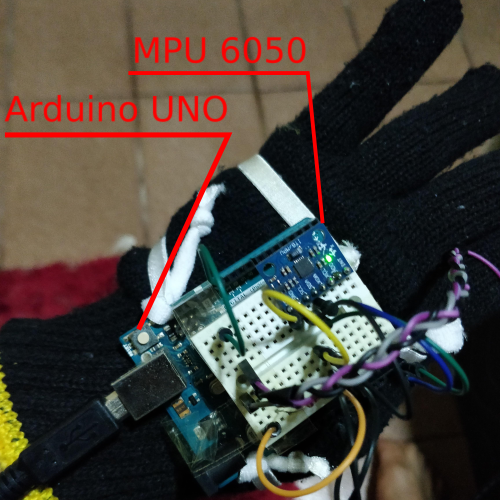
\includegraphics[width=0.4\textwidth]{resources/luva1.png}}
    \hfill
    \subfigure{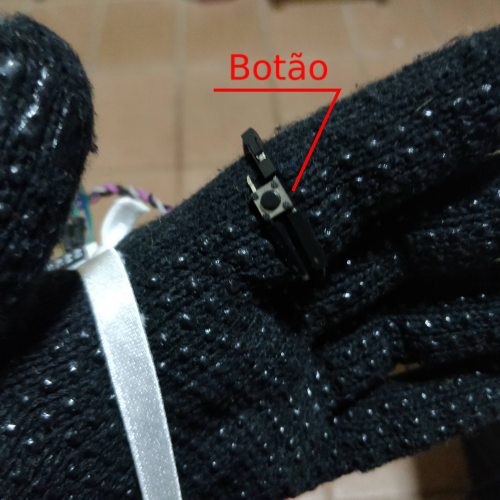
\includegraphics[width=0.4\textwidth]{resources/luva2.png}}
    \hfill
    \caption{Componentes da luva}
    \label{fig:luva}
\end{figure}

Os componentes são posicionados de maneira a garantir o máximo de conforto possível ao usuário. É recomendada a utilização de uma luva de pano para reduzir o contato do Arduino com a pele, pois os pontos de solda no verso da placa podem criar eventuais escoriações com a utilização prolongada do sistema. O Arduino deve ser posicionado no dorso da mão, preso com fitas elásticas firmes para evitar movimentações indesejadas que levariam à uma leitura imprecisa dos movimentos.

O sensor MPU 6050 está fixado em uma mini protoboard presa ao topo do Arduino com fitas adesivas de maneira estável. O botão de acionamento de captura de movimentos conta com os seus fios trançados afim aumentar a rigidez da construção do protótipo. Ao final da trança os fios são ligados ao botão de modo a formar um anel em volta do dedo indicador do usuário. Este posicionamento visa aumentar a ergonomia da luva, pois o botão estará convenientemente localizado no alcance do polegar do operador.

\subsubsection{Protótipo da central}

O esquemático da central apresentado na \autoref{fig:esq_central} do \autoref{chapter:metodo} define que a central é composta por um computador de propósito geral equipado com um microprocessador, capaz de executar algoritmos de aprendizado de máquina e enviar e receber sinais infravermelhos. Componentes com as mesmas funcionalidades dos propostos anteriormente foram utilizados no protótipo final, de maneira que foi possível validar o método proposto sem que fossem realizadas mudanças significativas.

O protótipo da central é composto por um \textit{Notebook}, conectado à luva através de uma conexão serial via cabo por uma porta USB, que processa os sinais recebidos e executa as ações correspondentes. Através de uma outra porta USB do \textit{Notebook}, uma outra conexão serial ligada à um segundo Arduino UNO, que atua como atuador, é realizada. Este Arduino faz o papel de receptor e emissor de sinais infravermelhos para o controle de dispositivos no ambiente. 

\begin{center}
    \missingfigure[figwidth=10cm]{Imagem da central}
\end{center}

\subsection{Análise do código-fonte do protótipo}

Existem três algoritmos sendo executados simultaneamente de maneira independente uns dos outros no protótipo, um no Arduino acoplado à luva, um no Arduino conectado à central e um na central em sí. Todos os códigos-fonte que são utilizados protótipo estão disponíveis gratuitamente em \url{https://github.com/JohnPinto/Hand.io}

\subsubsection{Análise dos algoritmos dos Arduinos}

Os algoritmos em execução nos dois Arduinos funcionam de maneira distinta. Durante a modelagem do sistema, foi definido que o Arduino presente na luva funcionaria apenas como sensor, enviando os sinais dos movimentos para a central, e o encontrado na central serviria de atuador, enviando os sinais infravermelhos para os dispositivos a serem controlados. Ambos os algoritmos foram implementados no dialeto de C/C++ utilizado na Arduido IDE próprio para codificação de Arduinos.

Durante o funcionamento nominal do sistema o Arduíno embutido na luva lê os sinais do sensor em tempo real, mas enquanto o botão de captura de movimentos presente na luva não for pressionado pelo usuário, é enviado para a central apenas uma sequência de pontos (.) com um curtíssimo intervalo de tempo entre os envios. 

Quando o botão é pressionado, a luva passa a enviar o sinal do acelerômetro e do giroscópio formatado  seguindo o padrão "\$    ax    ay    az    gx    gy    gz    " terminado com uma quebra de linha. O sinal é enviado desta maneira afim de garantir a consistência da transmissão dos dados. Este comportamento de envio intercalado de pontos (.) e sinais serve de condição de parada do algoritmo da central que será detalhado nas seções a seguir. Foi utilizada a biblioteca \textit{SoftwareSerial} para a realização de comunicação serial.

Já o Arduino conectado à central que serve de atuador, permanece ocioso até que um comando indicando qual sinal infravermelho deverá ser enviado seja recebido. Os códigos infravermelhos ficam armazenados diretamente no Arduino, graças ao desacoplamento dos códigos da memória RAM para a flash, isto permite ao usuário realizar o cadastro de centenas de códigos infravermelhos de dispositivos diferentes. 

Devido à natureza estacionária da central, é possível que múltiplos atuadores estejam inseridos em diversos cômodos diferentes de uma casa, por exemplo, o que serviria de aplicação para este trabalho. Na implementação deste algoritmo foram utilizadas as biblioteca \textit{SoftwareSerial} para comunicação serial, e \textit{IRremote}, para envio de sinais infravermelhos a partir do Arduino.

\subsubsection{Análise dos algoritmos da central}

\begin{figure}[ht]
    \centering
    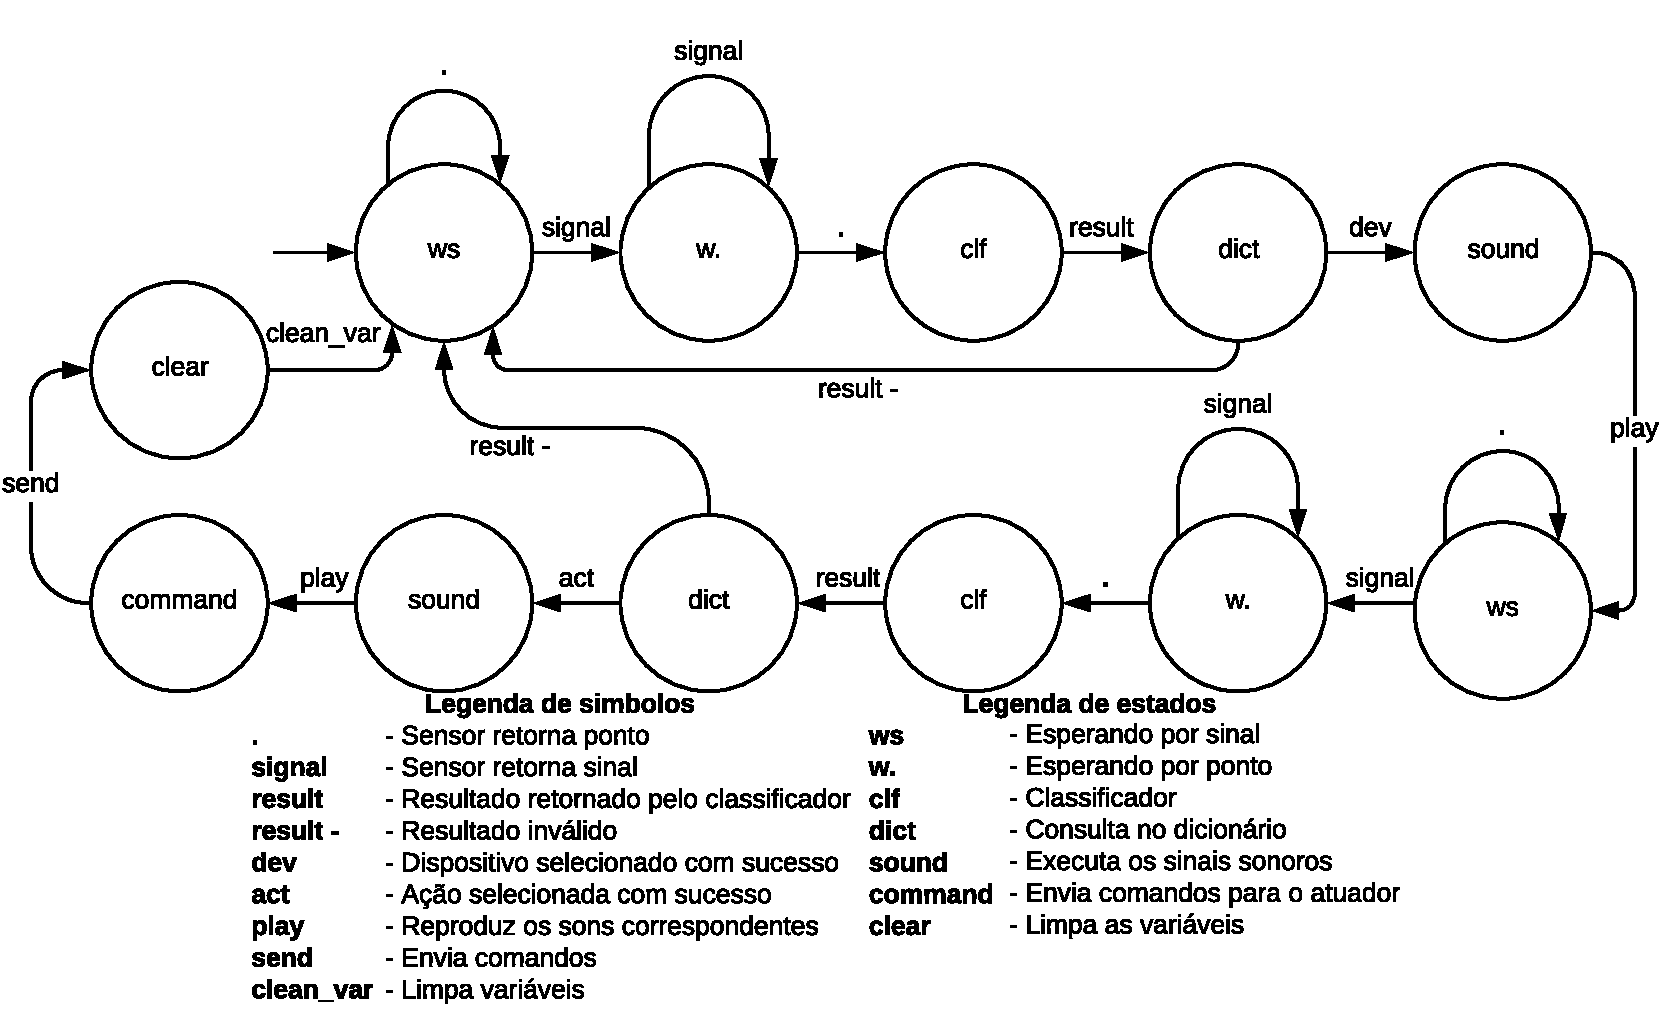
\includegraphics[width=\textwidth, keepaspectratio]{resources/maquina_estados.pdf}
    \caption{Máquina de estados da Hand.io}
    \label{fig:automato}
\end{figure}

O algoritmo aplicado na central de processamento tem o comportamento detalhado na \autoref{fig:automato}, que apresenta a máquina de estados que foi utilizada como modelo para a implementação da Hand.io. Graças à previsibilidade natural das máquinas de estados, o autor deste trabalho pôde isolar possíveis comportamentos indefinidos durante o desenvolvimento do projeto, o que reduziu consideravelmente o tempo de implementação do sistema. Os detalhes do diagrama serão discutidos em detalhes nas seções seguintes.

O código-fonte foi desenvolvido na linguagem de programação \textit{Python 3}, utilizando o paradigma de programação orientada a objetos, visando compartimentalizar o código com o objetivo de reduzir a imprevisibilidade, e evitar retrabalhos por parte do desenvolvedor. A linguagem em questão foi escolhida por sua praticidade de implementação devido à sua natureza de alto nível, o que permite uma implementação rápida e simples em comparação com as demais linguagens, além de contar com uma vasta gama de bibliotecas externas que agilizaram grandemente o desenvolvimento do protótipo.

\begin{figure}[ht]
    \centering
    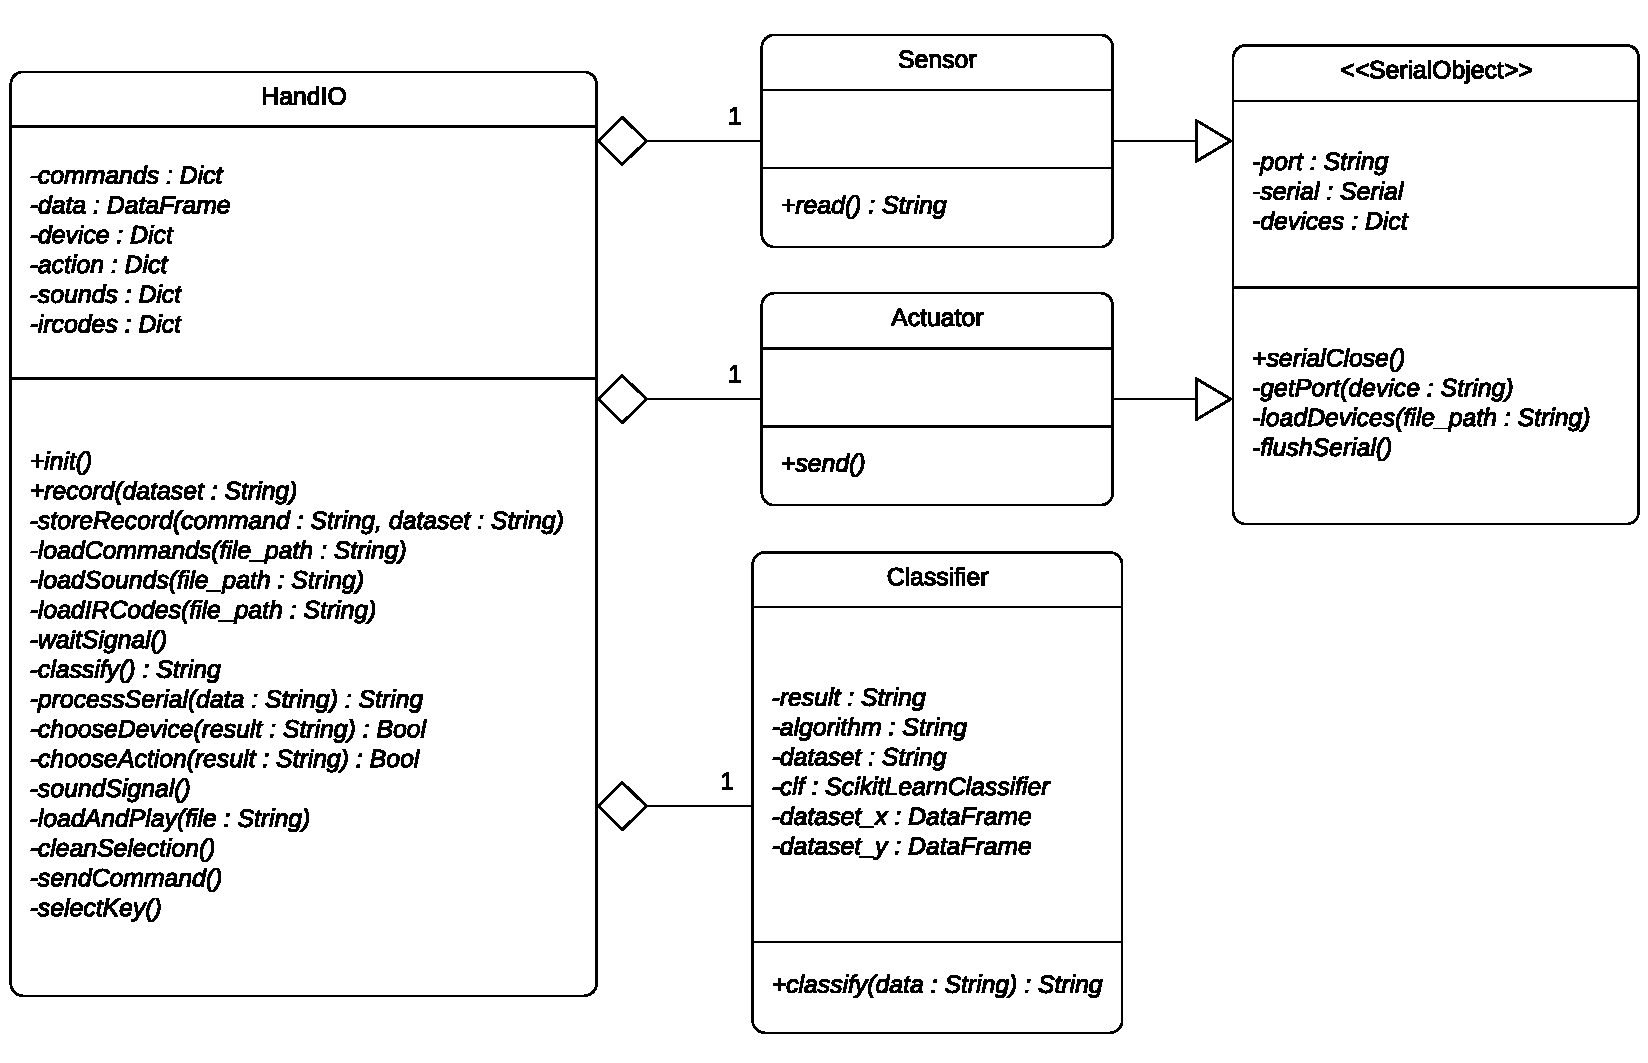
\includegraphics[width=\textwidth, keepaspectratio]{resources/diagrama_classe.pdf}
    \caption{Diagrama de classe da Hand.io}
    \label{fig:class}
\end{figure}

As especificidades da implementação podem ser vistas na \autoref{fig:class}, que detalha as relações entre as classes que compõem o sistema. A HandIO é a classe principal do programa, ela conta com diversos dicionários que agem como um especie de banco de dados rudimentar, esta abordagem foi escolhida para que haja a possibilidade do usuário modificar ou adicionar novos gestos ou dispositivos de maneira simplificada. Todos os dicionários utilizados são carregados a partir de arquivos correspondentes que podem ser encontrados na pasta json/ da pasta raiz do sistema. Foram implementados métodos privados que que iniciam com a palavra \textit{load}, que carregam cada dicionário individualmente, estes métodos são chamados no construtor do objeto.






\section{Planejamento e projeto do cenário experimental}

\subsection{Preparação do experimento}

\subsubsection{Componentes necessários}

\section{Execução do cenário experimental e análise dos resultados}

